\documentclass[sigconf]{acmart}
\usepackage{tikz}
\usetikzlibrary{shapes.geometric}
\usetikzlibrary{matrix}
\usetikzlibrary{graphs}
\usetikzlibrary{shapes.geometric}
\usepackage{pgfplots}
\pgfplotsset{compat=1.18} % Recommended for modern TikZ/pgfplots
\usepackage{environ}
\usepackage{ifthen}
\usepackage{graphicx}
\usepackage{subcaption}
\usepackage{fp}
\usepackage{makecell}
%%
%% \BibTeX command to typeset BibTeX logo in the docs
\AtBeginDocument{%
  \providecommand\BibTeX{{%
    Bib\TeX}}}

\setcopyright{acmlicensed}
\copyrightyear{2025}
\acmYear{2025}
\acmDOI{XXXXXXX.XXXXXXX}
%% These commands are for a PROCEEDINGS abstract or paper.
\acmConference[FPGA '26]{International Symposium on Field Programable Gate Arrays}{Febuary 22--24,
  2026}{Seaside, CA}
%%
%%  Uncomment \acmBooktitle if the title of the proceedings is different
%%  from ``Proceedings of ...''!
%%
%%\acmBooktitle{Woodstock '18: ACM Symposium on Neural Gaze Detection,
%%  June 03--05, 2018, Woodstock, NY}
\acmISBN{978-1-4503-XXXX-X/2018/06}

\begin{document}

\title{Multi-Port Memory with Bidirectional Ports for FPGAs Using XOR and LVT Methods}

%%
%% The "author" command and its associated commands are used to define
%% the authors and their affiliations.
%% Of note is the shared affiliation of the first two authors, and the
%% "authornote" and "authornotemark" commands
%% used to denote shared contribution to the research.
%\author{Kevin Townsend}
\author{XXX}
\email{XXX@XXX}

%\renewcommand{\shortauthors}{Townsend}
\renewcommand{\shortauthors}{XXX}

\begin{abstract}
  We propose a generalization to a previous XOR memory implementation to allow for any number of full, read-only, and write-only ports.
This implementation creates these additional ports by encoding and decoding the data entries with XOR logic. The incoming (written) data is encoded with the data corresponding to the other ports and the outgoing (read) data is decoded by XORing all the entries in the memory banks.
Using XOR operators to accomplish this encoding/decoding has advantages over other approaches because the XOR operator is a simple and efficient operation.
The result is a high-throughput multi-ported memory that is particularly well-suited for implementation on FPGAs.
This paper also presents an efficient architecture for creating a live value table (LVT) memory using an XOR-based scheme by utilizing its bidirectional capabilities.
We use an XOR memory with full ports to implement a bidirectional live value table design.
We evaluate the architecture's performance and resource utilization, and show that the XOR-based bidirectional live value table is a compelling alternative for applications requiring high-performance, flexible memory access.
\end{abstract}

%%
%% The code below is generated by the tool at http://dl.acm.org/ccs.cfm.
%% Please copy and paste the code instead of the example below.
%%
%\begin{CCSXML}
%<ccs2012>
% <concept>
%  <concept_id>00000000.0000000.0000000</concept_id>
%  <concept_desc>Do Not Use This Code, Generate the Correct Terms for Your Paper</concept_desc>
%  <concept_significance>500</concept_significance>
% </concept>
% <concept>
%  <concept_id>00000000.00000000.00000000</concept_id>
%  <concept_desc>Do Not Use This Code, Generate the Correct Terms for Your Paper</concept_desc>
%  <concept_significance>300</concept_significance>
% </concept>
% <concept>
%  <concept_id>00000000.00000000.00000000</concept_id>
%  <concept_desc>Do Not Use This Code, Generate the Correct Terms for Your Paper</concept_desc>
%  <concept_significance>100</concept_significance>
% </concept>
% <concept>
%  <concept_id>00000000.00000000.00000000</concept_id>
%  <concept_desc>Do Not Use This Code, Generate the Correct Terms for Your Paper</concept_desc>
%  <concept_significance>100</concept_significance>
% </concept>
%</ccs2012>
%\end{CCSXML}
%
%\ccsdesc[500]{Do Not Use This Code~Generate the Correct Terms for Your Paper}
%\ccsdesc[300]{Do Not Use This Code~Generate the Correct Terms for Your Paper}
%\ccsdesc{Do Not Use This Code~Generate the Correct Terms for Your Paper}
%\ccsdesc[100]{Do Not Use This Code~Generate the Correct Terms for Your Paper}

%%
%% Keywords. The author(s) should pick words that accurately describe
%% the work being presented. Separate the keywords with commas.
%\keywords{Do, Not, Us, This, Code, Put, the, Correct, Terms, for,
%  Your, Paper}
%% A "teaser" image appears between the author and affiliation
%% information and the body of the document, and typically spans the
%% page.

\received{1 Octomber 2025}
\received[revised]{XX XXX XXXX}
\received[accepted]{XX XXX XXXX}

%%
%% This command processes the author and affiliation and title
%% information and builds the first part of the formatted document.
\maketitle

\section{Motivation}

\begin{figure*}
  %\includegraphics[width=\textwidth]{sampleteaser}
  \centering
  %\begin{center}
  %\begin{scaletikzpicturetowidth}{\textwidth}
  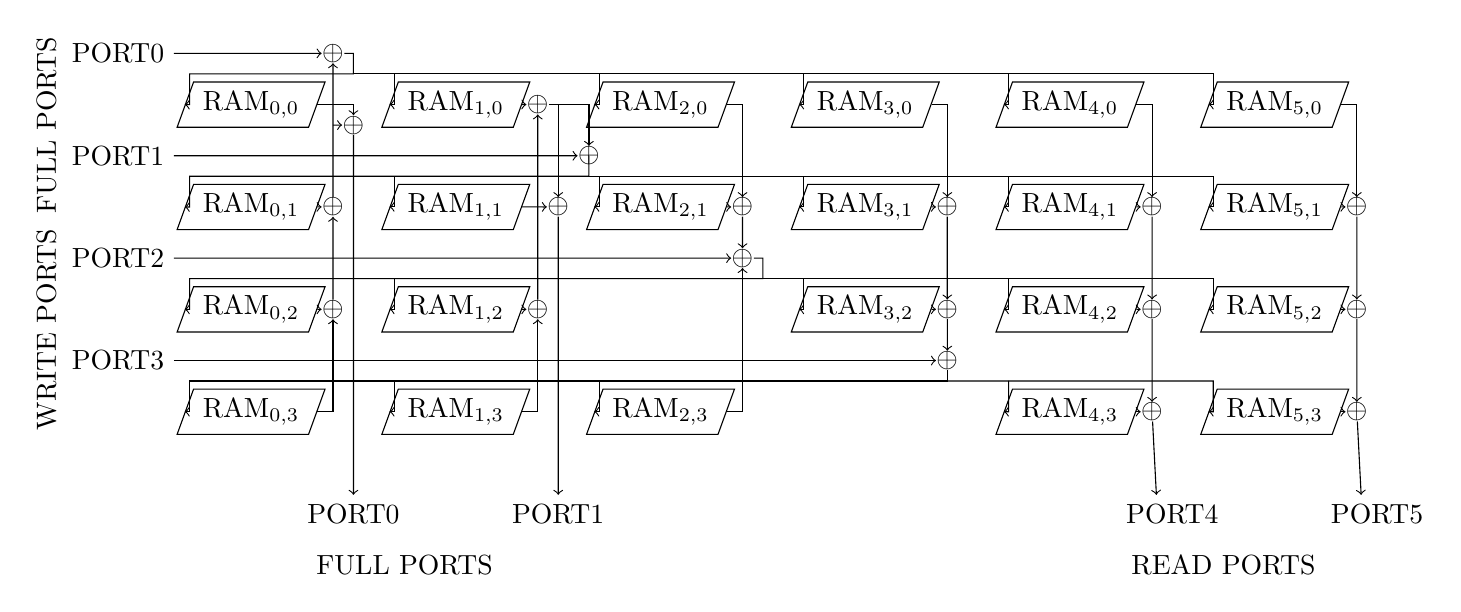
\begin{tikzpicture}[scale=1.3]
  \foreach \x in {0,1,2,3,4,5} {
    \foreach \y in {0,1,2,3} {
      \ifthenelse{\(\x = 2 \AND \y = 1\) \OR \(\x = 3 \AND \y = 0\)}{}{
        \node (r\x\y)[trapezium, trapezium left angle=70, trapezium right angle=110, draw] at (2*\x, \y){RAM$_{\x,\fpeval{3-\y}}$};
      }
    }
  }
  \foreach \x in {0,1,4,5} {
    \node (bport\x)[] at (2*\x+1, -1){PORT\x};
  }
  \foreach \y in {0,1,2,3} {
    \node (lport\y)[] at (-1.3, 3.5-\y){PORT\y};
  }
  \node [rotate=90] at (-2, .8){WRITE PORTS};
  \node [rotate=90] at (-2, 2.8){FULL PORTS};
  \node [] at (1.5, -1.5){FULL PORTS};
  \node [] at (9.5, -1.5){READ PORTS};
  \node(x50)[inner sep=0pt] at (10.8, 0){$\oplus$};
  \node(x51)[inner sep=0pt] at (10.8, 1){$\oplus$};
  \node(x52)[inner sep=0pt] at (10.8, 2){$\oplus$};
  \draw[->] (r50) -- (x50);
  \draw[->] (r51) -- (x51);
  \draw[->] (r52) -- (x52);
  \draw[->] (r53) -| (x52);
  \draw[->] (x52) -- (x51);
  \draw[->] (x51) -- (x50);
  \draw[->] (x50) -- (bport5.130);
  \node(x40)[inner sep=0pt] at (8.8, 0){$\oplus$};
  \node(x41)[inner sep=0pt] at (8.8, 1){$\oplus$};
  \node(x42)[inner sep=0pt] at (8.8, 2){$\oplus$};
  \draw[->] (r40) -- (x40);
  \draw[->] (r41) -- (x41);
  \draw[->] (r42) -- (x42);
  \draw[->] (r43) -| (x42);
  \draw[->] (x42) -- (x41);
  \draw[->] (x41) -- (x40);
  \draw[->] (x40) -- (bport4.130);
  \node(x31)[inner sep=0pt] at (6.8, 1){$\oplus$};
  \node(x32)[inner sep=0pt] at (6.8, 2){$\oplus$};
  \node(x30)[inner sep=0pt] at (6.8, .5){$\oplus$};
  \draw[->] (r31) -- (x31);
  \draw[->] (r32) -- (x32);
  \draw[->] (r33) -| (x32);
  \draw[->] (x32) -- (x31);
  \draw[->] (x31) -- (x30);
  %PORT3 connections.
  \draw[->] (lport3) -- (x30);
  \draw[->] (x30) |- (-.6,.3) |- (r00);
  \draw[->] (1.4,.3) |- (r10);
  \draw[->] (3.4,.3) |- (r20);
  \draw[->] (6.8, .3) -| (7.4,0) -- (r40);
  \draw[->] (7.4, .3) -| (9.4,0) -- (r50);
  %PORT2 XORs
  \node(x22)[inner sep=0pt] at (4.8, 2){$\oplus$};
  \node(x21)[inner sep=0pt] at (4.8, 1.5){$\oplus$};
  %PORT2 connections
  \draw[->] (lport2) -- (x21);
  \draw[->] (r23) -| (x22);
  \draw[->] (r22) -- (x22);
  \draw[->] (x22) -- (x21);
  \draw[->] (r20) -| (x21);
  \draw[->] (x21) -| (5,1.3) -| (-.6,1) -- (r01);
  \draw[->] (1.4,1.3) |- (r11);
  \draw[->] (5,1.3) -- (9.4, 1.3) |- (r51);
  \draw[->] (7.4, 1.3) |- (r41);
  \draw[->] (5.4, 1.3) |- (r31);
  %draw xor of full ports
  %PORT1
  \node(x11)[inner sep=0pt] at (2.8, 1){$\oplus$};
  \node(x12)[inner sep=0pt] at (3.3, 2.5){$\oplus$};
  \node(x12b)[inner sep=0pt] at (3, 2){$\oplus$};
  \node(x13)[inner sep=0pt] at (2.8, 3){$\oplus$};
  \draw[->] (r10) -| (x11);
  \draw[->] (r11) -- (x11);
  \draw[->] (lport1) -- (x12);
  \draw[->] (x11) -- (x13);
  \draw[->] (r13) -- (x13);
  \draw[->] (x13) -| (x12);
  \draw[->] (r12) -- (x12b);
  \draw[->] (x12) -| (3.3, 2.3) -| (-.6,2) -- (r02);
  \draw[->] (1.4,2.3) |- (r12);
  \draw[->] (3.3, 2.3) -- (9.4, 2.3) |- (r52);
  \draw[->] (3.4, 2.3) |- (r22);
  \draw[->] (5.4, 2.3) |- (r32);
  \draw[->] (7.4, 2.3) |- (r42);
  \draw[->] (x13) -| (x12b);
  \draw[->] (x12b) -- (bport1);
  %PORT0
  \node(x01)[inner sep=0pt] at (0.8, 1){$\oplus$};
  \node(x02)[inner sep=0pt] at (0.8, 2){$\oplus$};
  \node(x03)[inner sep=0pt] at (0.8, 3.5){$\oplus$};
  \node(x03b)[inner sep=0pt] at (1.0, 2.8){$\oplus$};
  \draw[->] (r00) -| (x01);
  \draw[->] (r01) -- (x01);
  \draw[->] (x01) -- (x02);
  \draw[->] (x02) -- (x03);
  \draw[->] (lport0) -- (x03);
  \draw[->] (x03) -| (1, 3.3) -| (-.6,3) -- (r03);
  \draw[->] (1, 3.3) -- (9.4, 3.3) |- (r53);
  \draw[->] (1.4, 3.3) |- (r13);
  \draw[->] (3.4, 3.3) |- (r23);
  \draw[->] (5.4, 3.3) |- (r33);
  \draw[->] (7.4, 3.3) |- (r43);
  \draw[->] (.8, 2.8) -- (x03b);
  \draw[->] (r02) -- (x02);
  \draw[->] (r03) -| (x03b);
  \draw[->] (x03b) -- (bport0);
  \end{tikzpicture}
  %\end{scaletikzpicturetowidth}
  %\end{center}
  \caption{A multi-port memory with 2 full ports, 2 write-only ports and 2 read-only ports.}
  \Description{Enjoying the baseball game from the third-base
  seats. Ichiro Suzuki preparing to bat.}
  \label{fig:teaser}
\end{figure*}
\begin{figure}
  \centering
  \begin{subfigure}[t]{0.45\textwidth}
    \centering
    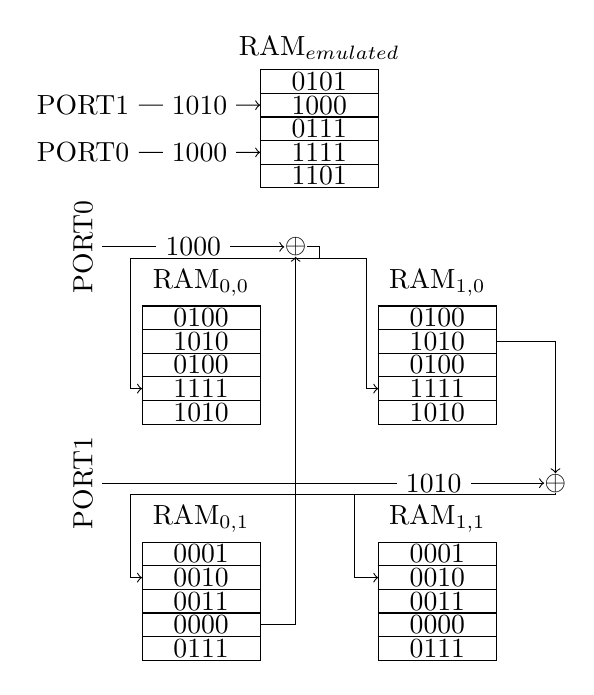
\begin{tikzpicture}[scale=3]
      \draw (.25,1.75) rectangle (.75,2.25);
      \foreach \j in {-.15,-.05, .05, .15}{
          \draw[] (.25, 2+\j) -- (.75,2+\j);
      }
      \foreach \i/\v in {0/1101,1/1111,2/0111,3/1000,4/0101}{
          \FPeval{\x}{.7-\i*.1};
          \FPeval{\y}{2-.2+\i*.1};
          \node[] at (.5,\y) {\v};
      }
      \node at (.5,2.25)[anchor=south]{RAM$_{emulated}$};
      \draw[xshift=-.5cm] (.25,0.75) rectangle (.75,1.25);
      \node at (0,1.25) [anchor=south]{RAM$_{0,0}$};
      \foreach \j in {-.15,-.05, .05, .15}{
          \draw[] (-.25, 1+\j) -- (.25,1+\j);
      }
      \foreach \i/\v in {0/1010,1/1111,2/0100,3/1010,4/0100}{
          \FPeval{\x}{.7-\i*.1};
          \FPeval{\y}{1-.2+\i*.1};
          \node[] at (0,\y) {\v};
      }
      \draw[xshift=.5cm] (.25,0.75) rectangle (.75,1.25);
      \node at (1,1.25) [anchor=south]{RAM$_{1,0}$};
      \foreach \j in {-.15,-.05, .05, .15}{
          \draw[] (1-.25, 1+\j) -- (1.25,1+\j);
      }
      \foreach \i/\v in {0/1010,1/1111,2/0100,3/1010,4/0100}{
          \FPeval{\y}{1-.2+\i*.1};
          \node[] at (1,\y) {\v};
      }
      \draw[xshift=-.5cm,yshift=-1cm] (.25,0.75) rectangle (.75,1.25);
      \node at (0,.25) [anchor=south]{RAM$_{0,1}$};
      \foreach \j in {-.15,-.05, .05, .15}{
          \draw[] (0-.25, 0+\j) -- (0.25,0+\j);
      }
      \foreach \i/\v in {0/0111,1/0000,2/0011,3/0010,4/0001}{
          \FPeval{\y}{1-.2+\i*.1};
          \node[] at (0,-1+\y) {\v};
      }
      \draw[xshift=.5cm,yshift=-1cm] (.25,0.75) rectangle (.75,1.25);
      \node at (1,.25) [anchor=south]{RAM$_{1,1}$};
      \foreach \j in {-.15,-.05, .05, .15}{
          \draw[] (1-.25, 0+\j) -- (1.25,0+\j);
      }
      \foreach \i/\v in {0/0111,1/0000,2/0011,3/0010,4/0001}{
          \FPeval{\y}{1-.2+\i*.1};
          \node[] at (1,-1+\y) {\v};
      }
      %draw XORs
      \node(x0)[inner sep=0pt] at (.4,1.5){$\oplus$};
      \node(x1)[inner sep=0pt] at (1.5,.5){$\oplus$};
      %draw ports
      \node(p0) at (-.5,1.5) [rotate=90]{PORT0};
      \node(p1) at (-.5,.5) [rotate=90]{PORT1};
      %draw connections
      \draw[->] (p1) -- (x1) node[pos=.75,fill=white]{1010};
      \draw[->] (1.25,1.1) -| (x1);
      \draw (x1) |- (-.3, .45);
      \draw[->] (-.3, .45) |- (-.25, 0.1);
      \draw[->] (.65, .45) |- (.75, 0.1);
      \draw[->] (p0) -- (x0) node[pos=.5,fill=white]{1000};
      \draw[->] (.25,-.1) -| (x0);
      \draw[->] (x0) -| (.5,1.45) -| (-.3, .9) -- (-.25, .9);
      \draw[->] (.5,1.45) -| (.7, .9) -- (.75, .9);
      % draw emulated ram connections.
      \node(ep1) at (-.5,2.1) {PORT1};
      \draw[->] (ep1) -- (.25,2.1) node[midway,fill=white]{1010};
      \node(ep0) at (-.5,1.9) {PORT0};
      \draw[->] (ep0) -- (.25,1.9) node[midway,fill=white]{1000};
    \end{tikzpicture}
    \caption{The memory on clock cycle 0, where $1000_2$ is written to address 1 from port 0 and $1010_2$ is written to address 3 from port 1.}

  \end{subfigure}
  \begin{subfigure}[t]{0.45\textwidth}
    \centering
    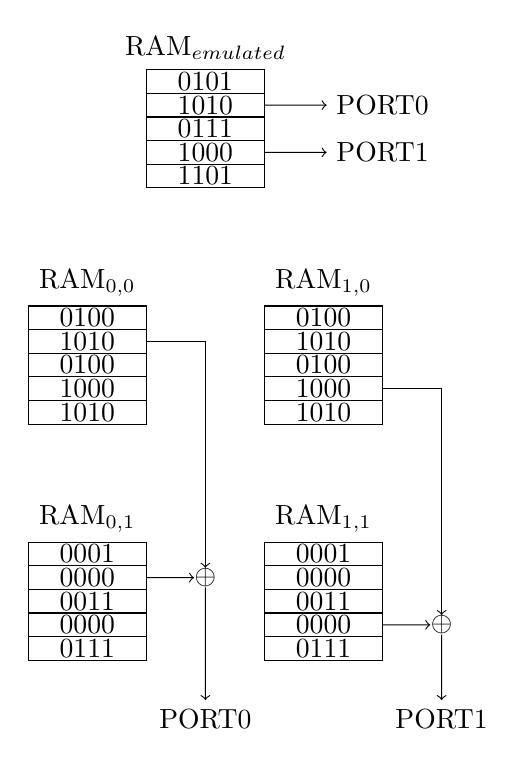
\begin{tikzpicture}[scale=3]
      %draw emulated ram
      %\draw[] (.5,2-.25) -- (1,2-.25) -- (.5,2.25) -- (0, 2.25) -- cycle;
      \draw (.25,1.75) rectangle (.75,2.25);
      \foreach \j in {-.15,-.05, .05, .15}{
          \draw[] (.25, 2+\j) -- (.75,2+\j);
      }
      \foreach \i/\v in {0/1101,1/1000,2/0111,3/1010,4/0101}{
          \FPeval{\x}{.7-\i*.1};
          \FPeval{\y}{2-.2+\i*.1};
          \node[] at (.5,\y) {\v};
      }
      \node at (.5,2.25)[anchor=south]{RAM$_{emulated}$};
      \draw[xshift=-.5cm] (.25,0.75) rectangle (.75,1.25);
      \node at (0,1.25) [anchor=south]{RAM$_{0,0}$};
      \foreach \j in {-.15,-.05, .05, .15}{
          \draw[] (-.25, 1+\j) -- (.25,1+\j);
      }
      \foreach \i/\v in {0/1010,1/1000,2/0100,3/1010,4/0100}{
          \FPeval{\x}{.7-\i*.1};
          \FPeval{\y}{1-.2+\i*.1};
          \node[] at (0,\y) {\v};
      }
      \draw[xshift=.5cm] (.25,0.75) rectangle (.75,1.25);
      \node at (1,1.25) [anchor=south]{RAM$_{1,0}$};
      \foreach \j in {-.15,-.05, .05, .15}{
          \draw[] (1-.25, 1+\j) -- (1.25,1+\j);
      }
      \foreach \i/\v in {0/1010,1/1000,2/0100,3/1010,4/0100}{
          \FPeval{\y}{1-.2+\i*.1};
          \node[] at (1,\y) {\v};
      }
      \draw[xshift=-.5cm,yshift=-1cm] (.25,0.75) rectangle (.75,1.25);
      \node at (0,.25) [anchor=south]{RAM$_{0,1}$};
      \foreach \j in {-.15,-.05, .05, .15}{
          \draw[] (0-.25, 0+\j) -- (0.25,0+\j);
      }
      \foreach \i/\v in {0/0111,1/0000,2/0011,3/0000,4/0001}{
          \FPeval{\y}{1-.2+\i*.1};
          \node[] at (0,-1+\y) {\v};
      }
      \draw[xshift=.5cm,yshift=-1cm] (.25,0.75) rectangle (.75,1.25);
      \node at (1,.25) [anchor=south]{RAM$_{1,1}$};
      \foreach \j in {-.15,-.05, .05, .15}{
          \draw[] (1-.25, 0+\j) -- (1.25,0+\j);
      }
      \foreach \i/\v in {0/0111,1/0000,2/0011,3/0000,4/0001}{
          \FPeval{\y}{1-.2+\i*.1};
          \node[] at (1,-1+\y) {\v};
      }
      %add ports
      \node(p0) at (.5,-.5) {PORT0};
      % add xors
      \node(x0)[inner sep=0pt] at (.5,0.1){$\oplus$};
      %add connections
      \draw[->] (.25, 1.1) -| (x0);
      \draw[->] (.25, .1) -- (x0);
      \draw[->] (x0) -- (p0);
      %add ports
      \node(p1) at (1.5,-.5) {PORT1};
      %add xors
      \node(x1)[inner sep=0pt] at (1.5,-.1){$\oplus$};
      %add connections
      \draw[->] (1.25, .9) -| (x1);
      \draw[->] (1.25, -.1) -- (x1);
      \draw[->] (x1) -- (p1);
      %add emulated ports
      \node(ep0) at (1.25, 2.1) {PORT0};
      \node(ep1) at (1.25, 1.9) {PORT1};
      \draw[->] (.75,2.1) -- (ep0);
      \draw[->] (.75,1.9) -- (ep1);
    \end{tikzpicture}
    \caption{The memory on clock cycle 1, where $1010_2$ is read from address 3 from port 0 and $1000_2$ is read from address 1 from port 1.}
  \end{subfigure}
  \caption{This shows an XOR memory during 2 clock cycles of operation. The XOR memory has 2 full ports and is constructed from 4 RAMs with 1 read and 1 write port.}
  \label{fig:xor_example}
  \Description{An illustration.}
\end{figure}


As computation needs keep increasing, one way to keep up has been
specialized architectures. FPGAs provide a way to implement such architectures without taping out an ASIC.
However, the limitations of FPGA resources requires some creativity to map designs to FPGAs.
This paper explores how to overcome the limitation that FPGA memories have a limited number of
ports. Specifically, we propose a method to create memories with more than 2 ports.

The major FPGA vendors (AMD\cite{amd20}, Intel\cite{intel24}, Lattice\cite{lattice21}, Micro\-chip\cite{microchip_polarfire_fabric}, and Achronix\cite{achronix_ds015}) implement distributed memory (small memories) and block memory (large memories)
differently. However they all share some characteristics. All vendors support distributed memory configurations with 1 full or write port and between 1 to 3 read ports. All vendors support block memory with 2 full ports. AMD has a limited offering of multi-port memories, but otherwise none of the vendors support memories with more than 2 full ports. Although this limitation is problematic for designs requiring multiple ports (and particularly write or full ports), we show that these resources can be configured to achieve high throughput full port memories.

\section{Source Code}
We provide all of the source code used in implementation and testing our design at
https://anonymous.4open.science/r/mpm-7666/. We tested our design with Verilator\cite{verilator_manual} and synthesized the design
with Vivado\cite{ug893} targeting an AMD Virtex UltraScale+ HBM VU47P-3 FPGA.

\section{Related Work}

Several previous solutions to the port limit of FPGA memories exist, including multi-pumping, banking and replication\cite{laforest10}. Multi-pumping is the process of reducing
the clock speed to increase the number of ports. For example, a 300Mhz single
port memory can handle two 150Mhz ports. Banking\cite{townsend15} requires stalls and routing logic
due to the segmented memory. Our design is most similar to replication. Replication involves tying the write ports of multiple memories together to create additional read ports.

\section{Generalizing XOR memory}

We propose a simple generalization to XOR memories presented in previous work\cite{laforest14}.
XOR memories work by using the following property:
\begin{equation} \label{eqn:xor}
a \oplus b \oplus b = a
\end{equation}
Where $\oplus$ is the bitwise XOR operator. Equation 1 follows from:
\begin{equation}
a \oplus 0 = a
\end{equation}
and
\begin{equation}
a \oplus a = 0
\end{equation}
Meaning XOR is the inverse operator of itself. Combined with the commutative and associative property of XOR we can generalize this to:
\begin{equation}
b_0 \oplus \dots \oplus b_n \oplus (a \oplus b_0 \dots \oplus b_n) = a
\end{equation}

This implementation creates these additional ports by encoding and decoding the entries with XOR logic. The incoming (written) data is encoded with the data corresponding to the other ports, and the outgoing (read) data is decoded by XORing all the entries in the memory banks. Using XOR operators to accomplish this encoding/decoding has advantages over other approaches, because the XOR operator is simply and efficiently implemented with LUTs.

We use XOR logic to add bidirectional
ports and analyze the performance of distributed memory and block memory
versions of this design.

Figure \ref{fig:teaser} demonstrates how to create an XOR memory with 2 read ports, 2 write ports and 2 full ports, which requires 22 RAMs. To read data from an XOR memory all of the data from the RAMs in one column is XORed from the same address. For example, say address $x$ has values $A$, $B$, $C$ and $D$, the data read would be $A\oplus B\oplus C \oplus D$.

Writing to the memory involves reading from all memories except the current row (e.g., say row/port 2 in Figure \ref{fig:teaser}) and XORing the incoming data $E$, (in the example this results in $A\oplus B \oplus D \oplus E$) and storing that value in all the RAMs in that row.
The next time that data is read the result will be $A\oplus B \oplus (A \oplus B\oplus D\oplus E) \oplus D$, which equals $E$.

Note that writing to a port involves XORing all but one stored value and reading involves XORing all values. This enables full ports to be created just by adding one RAM to what would otherwise be just a write port.

The number of RAMs ($N_{RAM}$) needed for this memory is:
\begin{equation}
N_{RAM}=(W+F)(W+F+R)-W
\end{equation}
Where $W$ is the number of write ports, $R$ is the number of read ports and $F$ is the number of full ports. This expands to:
\begin{equation}
N_{RAM}=W^2 + 2WF + F^2 + WR + FR - W
\end{equation}

Note that this memory requires that all of the RAMs in a row have the same data. Initializing the rams to the same data (e.g., all 0s) is required for the memory to operate properly. This is not an issue in FPGAs since the memory can be initialized to 0. Since rows are written to at the same time, they will remain the same as long as the memories are initially the same.

We provide a second example with Figure \ref{fig:xor_example} showing two clock cycles of operation of an XOR memory with 2 full ports. We use 2 ports for simplicity. These examples can be extrapolated to more ports.

\section{Analysis of XOR Memory Performance}

We analyze several configurations of XOR memories in terms of resource usage. Tables \ref{tab:syn_xor_ports} through \ref{tab:syn_xor_bram_ports} present some sample performance characteristics, including usage of look up tables (LUTs), flip-flops (FFs), block RAMs (BRAMs) and the maximum frequency that can be achieved under variations of number of ports and the width and depth of the memory.

Table \ref{tab:syn_xor_ports} shows the varying resources and max frequency of the memory for different numbers of ports. As seen the number of LUTs used for memory is relatively large and particularly large for more ports. We use 2, 4, 8, 16, and 32 ports although there is no limitation for using other port counts (3, 5, 6, 7, etc.). As shown, the resource usage increases quadradically with the number of ports.

Table \ref{tab:syn_xor_width} shows the varying resources and max frequency of the memory for different widths. As expected increasing the width of the memory resulted in a roughly linear increase in resource usage and a decrease in timing performance.

Table \ref{tab:syn_xor_depth} shows the varying resources and max frequency of the memory for different memory depths. Also as expected, increasing the depth of the memory resulted in a roughly linear increase in resource usage and a decrease in timing performance.

Table \ref{tab:syn_xor_bram_ports} shows results from an implementation using block RAMs. This required changing the block RAM to be write before read to remove the cycle of write delay. As shown the block RAM usage increases quadratically with the number of ports.

\begin{table}
  \caption{Synthesis results of XOR memory for different port counts. Each memory has a depth of 1024 and width of 32 bits. To reduce the number of IO ports and fit the design on the FPGA, we used a wrapper for the multi-port memory for the design with 16 ports. The 32 port design used more resources than are available on the FPGA therefore we do not have timing for that design.}
  \label{tab:syn_xor_ports}
  \begin{tabular}{llllll}
    \toprule
    Ports & LUTs & \thead{LUTs\\ configured\\ as memory} & FFs & BRAMs & Max Frequency\\
    \midrule
    2 & 2,920 & 2,432 & 0 & 0 & 625Mhz\\
    4 & 12,496 & 10,496 & 0 & 0 & 500Mhz\\
    8 & 52,128 & 43,520 & 0 & 0 & 357Mhz\\
    16 & 212,288 & 177,152 & 0 & 0 & 150Mhz\\
    32 & 858,752 & 714,752 & 0 & 0 & N/A\\
    \bottomrule
  \end{tabular}
\end{table}

\begin{table}
  \caption{Synthesis results of XOR memory for different widths. Each memory has a depth of 1024 and 8 ports.}
  \label{tab:syn_xor_width}
  \begin{tabular}{llllll}
    \toprule
    Width & LUTs & \thead{LUTs\\ configured\\ as memory} & FFs & BRAMs & Max Frequency\\
    \midrule
    1 & 2,168 & 1,920 & 0 & 0 & 526Mhz\\
    2 & 4,240 & 3,840 & 0 & 0 & 500Mhz\\
    4 & 7,104 & 5,888 & 0 & 0 & 400Mhz\\
    8 & 14,048 & 11,776 & 0 & 0 & 385Mhz\\
    16 & 26,144 & 21,760 & 0 & 0 & 370Mhz\\
    32 & 52,128 & 43,520 & 0 & 0 & 357Mhz\\
    \bottomrule
  \end{tabular}
\end{table}

\begin{table}
  \caption{Synthesis results of XOR memory for different depths. Each memory has a width of 32 bits and 8 ports.}
  \label{tab:syn_xor_depth}
  \begin{tabular}{llllll}
    \toprule
    Depth & LUTs & \thead{LUTs\\ configured\\ as memory} & FFs & BRAMs & Max Frequency\\
    \midrule
    32 & 2,368 & 1,600 & 0 & 0 & 588Mhz\\
    64 & 3,488 & 2,720 & 0 & 0 & 556Mhz\\
    128 & 6,864 & 5,440 & 0 & 0 & 526Mhz\\
    256 & 13,472 & 10,880 & 0 & 0 & 476Mhz\\
    512 & 26,576 & 21,760 & 0 & 0 & 455Mhz\\
    1,024 & 52,128 & 43,520 & 0 & 0 & 357Mhz\\
    \bottomrule
  \end{tabular}
\end{table}

\begin{table}
  \caption{Synthesis results of XOR memory with block RAMs for different port counts. Each memory has a depth of 1024 and width of 32 bits. To reduce the number of IO ports and fit the design on the FPGA, we used a wrapper for the multi-port memory for designs with 16 and 32 ports.}
  \label{tab:syn_xor_bram_ports}
  \begin{tabular}{llllll}
    \toprule
    Ports & LUTs & \thead{LUTs\\ configured\\ as memory} & FFs & BRAMs & Max Frequency\\
    \midrule
    2 & 144 & 0 & 218 & 4 & 625Mhz\\
    4 & 512 & 0 & 444 & 16 & 476Mhz\\
    8 & 1920 & 0 & 920 & 64 & 370Mhz\\
    16 & 6,656 & 0 & 1,968 & 256 & 263Mhz\\
    32 & 10,240 & 0 & 2,400 & 1024 & 123Mhz\\
    \bottomrule
  \end{tabular}
\end{table}

\section{Live Value Table Memory}
\begin{figure}
  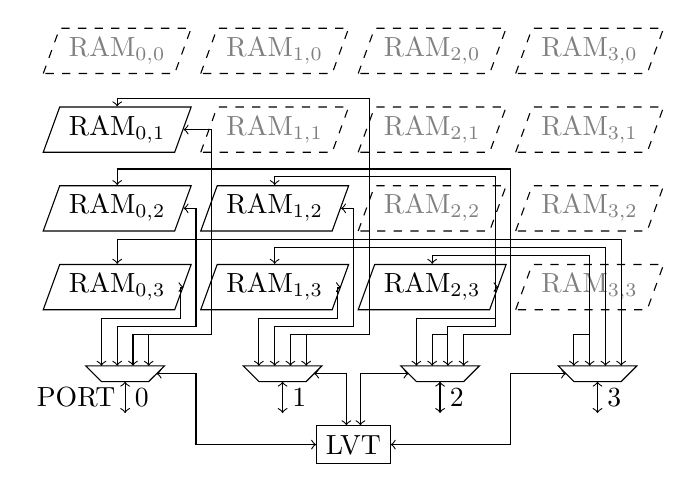
\begin{tikzpicture}[xscale=2]
  %draw rams
  \foreach \x in {0,1,2,3} {
    \foreach \y in {0,1,2,3} {
      \ifthenelse{\x < \y}{
      \node(r\y\x)[trapezium, trapezium left angle=70, trapezium right angle=110, draw] at (\x,3-\y) {RAM$_{\x,\y}$};
      }{
      \node[text=gray,dashed, trapezium, trapezium left angle=70, trapezium right angle=110, draw] at (\x,3-\y) {RAM$_{\x,\y}$};
      }
    }
  }
  %draw a ports
  \foreach \x in {0,1,2,3} {
    %\node(xport\x) at (\x, -1) {\x};
  }
  %draw b ports
  \foreach \y in {0,1,2,3} {
    %\node(yport\y) at (-1, 3-\y) {\y};
  }
  %draw connections
  \draw[<->] (r10.east) -| (.6,-.6) -| (.1,-1);
  \draw[->] (.2,-.6) -- (.2,-1);
  \draw[<->] (r20.east) -| (.5,-.5) -| (.0,-1);
  \draw[<->] (r30.east) -| (.4,-.4) -| (-.1,-1);
  \draw[<->] (r10) |- (1.6, 2.4) |- (1.2, -.6) -- (1.2,-1);
  \draw[->] (1.2,-.6) -| (1.1,-1);
  \draw[<->] (r21) -| (1.5,-.5) -| (1,-1);
  \draw[<->] (r31) -| (1.4,-.4) -| (.9,-1);
  \draw[<->] (r20) |- (2.5,1.5) |- (2.2, -.6) -- (2.2,-1);
  \draw[<->] (r21) |- (2.4,1.4) |- (2.1, -.5) -- (2.1,-1);
  \draw[->] (2.1,-.6) -| (2.0,-1);
  \draw[<->] (r32) -| (2.4,-.4) -| (1.9,-1);
  \draw[<->] (r30) |- (3.2,.6) -- (3.2,-1);
  \draw[<->] (r31) |- (3.1,.5) -- (3.1,-1);
  \draw[<->] (r32) |- (3.0,.4) -- (3.0,-1);
  \draw[->] (3.0,-.6) -| (2.9,-1);
%  %x0 connections
%  \draw (xport0) .. controls (.8,-1) and (.8,2) .. (r10.east);
%  \draw (xport0) .. controls (.6,-1) and (.7,1) .. (r20.east);
%  \draw (xport0) .. controls (.4,-1) and (.6,0) .. (r30.east);
%  %x1 connections
%  \draw (xport1) .. controls (1.6,-1) and (1.7,1) .. (r21);
%  \draw (xport1) .. controls (1.4,-1) and (1.6,0) .. (r31);
%  %x2 connection
%  \draw (xport2) .. controls (2.4,-1) and (2.6,0) .. (r32);
%  %y1 connection
%  \draw (yport1) .. controls (-1, 2.5) and (0, 2.5) .. (r10);
%  %y2 connections
%  \draw (yport2) .. controls (-1, 1.4) and (0, 1.4) .. (r20);
%  \draw (yport2) .. controls (-1, 1.6) and (1, 1.6) .. (r21);
%  %y3 connections
%  \draw (yport3) .. controls (-1, 0.4) and (0, 0.4) .. (r30);
%  \draw (yport3) .. controls (-1, 0.6) and (1, 0.6) .. (r31);
%  \draw (yport3) .. controls (-1, 0.8) and (2, 0.8) .. (r32);
%  %draw labels
%  \node at (-1.5, 1)[rotate=90]{Ports};
%  \node at (1, -1.5){Ports};
  %draw muxes
  \draw[xshift=-.2cm,yshift=-1cm] (0,0) -- (.1,-.2) -- (.4,-.2) -- (.5,0) -- cycle;
  \draw[xshift=.8cm,yshift=-1cm] (0,0) -- (.1,-.2) -- (.4,-.2) -- (.5,0) -- cycle;
  \draw[xshift=1.8cm,yshift=-1cm] (0,0) -- (.1,-.2) -- (.4,-.2) -- (.5,0) -- cycle;
  \draw[xshift=2.8cm,yshift=-1cm] (0,0) -- (.1,-.2) -- (.4,-.2) -- (.5,0) -- cycle;
  %draw LVT
  \node(lvt)[draw] at (1.5, -2) {LVT};
  %draw LVT connections
  \draw[<->] (lvt) -- (.5,-2) |- (.25,-1.1);
  \draw[<->] (lvt.110) |- (1.25,-1.1);
  \draw[<->] (lvt.70) |- (1.85,-1.1);
  \draw[<->] (lvt) -- (2.5,-2) |- (2.85,-1.1);
  %draw ports
  \node[anchor=east] at (.05,-1.4) {PORT};
  \draw[<->] (.05,-1.2) -- (.05,-1.6) node[right,midway]{0};
  \draw[<->] (1.05,-1.2) -- (1.05,-1.6) node[right,midway]{1};
  \draw[<->] (2.05,-1.2) -- (2.05,-1.6) node[right,midway]{2};
  \draw[<->] (3.05,-1.2) -- (3.05,-1.6) node[right,midway]{3};
  \end{tikzpicture}
 \caption{Multi-port memory created with bidirectional dual-port RAMs. Note, a live value table is needed to determine which RAM has the most recent value.}
  \label{fig:lvt0}
  \Description{An illustration.}
\end{figure}

%\begin{figure}
%  \begin{tikzpicture}[yscale=1.2]
%    \node(lvt)[draw] at (2.5, 1) {LVT};
%    \foreach \x in {0,1,2,3}{
%    \node(mux\x)[draw,trapezium, rotate=-90,inner sep=5pt] at (2*\x,0){};
%    \node(mux\x port0) at (2*\x-.7,.3){0};
%    \node(mux\x port1) at (2*\x-.7,.1){1};
%    \node(mux\x port2) at (2*\x-.7,-.1){2};
%    \node(mux\x port3) at (2*\x-.7,-.3){3};
%    \ifthenelse{\x=0}{
%    \draw[->,dashed] (mux\x port0) -- (mux\x.210);
%    }{
%    \draw[->] (mux\x port0) -- (mux\x.210);
%    }
%    \ifthenelse{\x=1}{
%    \draw[->,dashed] (mux\x port1) -- (mux\x.240);
%    }{
%    \draw[->] (mux\x port1) -- (mux\x.240);
%    }
%    \ifthenelse{\x=2}{
%    \draw[->,dashed] (mux\x port2) -- (mux\x.300);
%    }{
%    \draw[->] (mux\x port2) -- (mux\x.300);
%    }
%    \ifthenelse{\x=3}{
%    \draw[->,dashed] (mux\x port3) -- (mux\x.330);
%    }{
%    \draw[->] (mux\x port3) -- (mux\x.330);
%    }
%    \draw[->] (mux\x ) -- (2*\x+.5,0);
%    \node at (2*\x,-.5) {PORT\x};
%    }
%    \draw[->] (lvt) .. controls (0,.5) .. (mux0);
%    \draw[->] (lvt) .. controls (2,.5) .. (mux1);
%    \draw[->] (lvt) .. controls (4,.5) .. (mux2);
%    \draw[->] (lvt) .. controls (6,.5) .. (mux3);
%  \end{tikzpicture}
%  \caption{The live value table for the memory in figure \ref{fig:lvt0}.}
%  \Description{An illustration.}
%\end{figure}

XOR memories can be used by themselves, but combining a live value table (LVT) with XOR may be more efficient. We present a LVT memory that utilizes XOR memory.

In an alternate implementations\cite{laforest12}\cite{choi12}, the live value table was implemented with registers. Previous work has used distributed memory \cite{abdelhadi16}. However, that work did not use a bidirectional XOR memory in their implementation.

We create a LVT memory using the technique described in \cite{choi12}. This LVT memory is composed of bidirectional dual-port RAMs. Each port of the LVT memory shares a RAM with another port of the LVT memory. This results in $F(F-1)/2$ RAMs being needed, where $F$ is the number of bidirectional (full) ports. This is less than the $F^2$ RAMs needed in the XOR implementation. Figure \ref{fig:lvt0} illustrates the implementation for 4 ports.

The memory gets its name because it uses multi-port memory to track the most recent stored value (i.e., a live value table). The point of a multi-port memory that requires a multi-port memory is that wide (e.g., 32 bit data) can be stored more efficiently this way, since the live value table is just storing the port numbers. (e.g., In Figure \ref{fig:lvt0} the live value table memory has a width of 2 since there are 4 ports.)

\section{Analysis of LVT Memory}

We explore LVT designs with 2 to 32 ports. Although 16 and 32 port designs can fit on large FPGAs, we believe smaller 3 to 8 port designs are more practical. We say
more practical because of the high resource usage of XOR and LVT memories at high port counts:
$F^2$ for XOR and $F(F-1)/2$ for LVT. However, we were able to synthesize a 32 port memory. Higher port counts also had worse timing performance (see Table \ref{tab:syn} and Figure \ref{fig:lvt_frequency}).

Table \ref{tab:syn} shows the varying resources and max frequency of the memory for different numbers of ports.

%TODO: elaborate on table and figures.

To get better timing performance, we created a pipelined version of the memory. This memory has major drawbacks: In addition to read delay the memory has write delay. The write delay means write conflicts occur on adjacent clock cycles and not just current clock cycles. However, we achieve better timing performance with this memory (see Table \ref{tab:syn_pipelined} and Figure \ref{fig:lvt_frequency}).

Table \ref{tab:syn_pipelined} shows the varying resources and max frequency of the memory for different numbers of ports.

Without write delay an 8 port memory runs at 455mhz (63\% of max frequency of the block RAM). With write delay and pipelining an 8 port memory design runs at 625mhz (87\% of max frequency of the block RAM).

\begin{figure}
  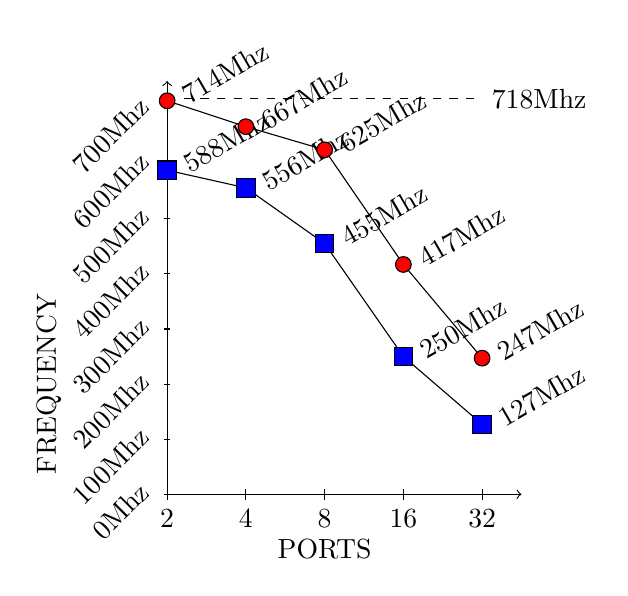
\begin{tikzpicture}[yscale=.7]
    \draw[->] (0,0) -- (4.5, 0);
    \draw (0,.1) -- (0, -.1) node[anchor=north] {2};
    \draw (1,.1) -- (1, -.1) node[anchor=north] {4};
    \draw (2,.1) -- (2, -.1) node[anchor=north] {8};
    \draw (3,.1) -- (3, -.1) node[anchor=north] {16};
    \draw (4,.1) -- (4, -.1) node[anchor=north] {32};
    %draw y axis
    \draw[->] (0,0) -- (0, 7.5);
    \draw (1pt, 0) -- (-1pt, 0) node[rotate=45,anchor=south east] {0Mhz};
    \foreach \y in {1,2,3,4,5,6,7}
      \draw (1pt, \y) -- (-1pt, \y) node[rotate=45,anchor=south east] {\y00Mhz};
    %labels
    \node at (2,-1) {PORTS};
    \node at (-1.5,2) [rotate=90]{FREQUENCY};
    %max frequncy
    \draw[dashed] (0, 7.18) -- (4, 7.18) node[anchor=west] {718Mhz};
    %line graphs
    \draw (0, 5.88) -- (1, 5.56) -- (2, 4.55) -- (3, 2.50) -- (4, 1.27);
    \node[fill=blue, draw,label={[rotate=30]right:588Mhz}] at (0,5.88){};
    \node[fill=blue, draw,label={[rotate=30]right:556Mhz}] at (1,5.56){};
    \node[fill=blue, draw,label={[rotate=30]right:455Mhz}] at (2,4.55){};
    \node[fill=blue, draw,label={[rotate=30]right:250Mhz}] at (3,2.50){};
    \node[fill=blue, draw,label={[rotate=30]right:127Mhz}] at (4,1.27){};
    %line graph for pipelnined.
    \draw (0, 7.14) -- (1, 6.67) -- (2, 6.25) -- (3, 4.17) -- (4, 2.47);
    \node[fill=red, draw, circle,inner sep=2pt,label={[rotate=30]right:714Mhz}] at (0,7.14){};
    \node[fill=red, draw, circle,inner sep=2pt,label={[rotate=30]right:667Mhz}] at (1,6.67){};
    \node[fill=red, draw, circle,inner sep=2pt,label={[rotate=30]right:625Mhz}] at (2,6.25){};
    \node[fill=red, draw, circle,inner sep=2pt,label={[rotate=30]right:417Mhz}] at (3,4.17){};
    \node[fill=red, draw, circle,inner sep=2pt,label={[rotate=30]right:247Mhz}] at (4,2.47){};
  \end{tikzpicture}
  \caption{Frequency of LVT design. The \protect\tikz{\protect\node[fill=blue, draw]{}}s are the (non-pipelined) LVT memory designs and the \protect\tikz{\protect\node[fill=red, draw, circle,inner sep=2pt]{}}s are the pipelined LVT memory designs.}
  \label{fig:lvt_frequency}
  \Description{A graph showing the frequency of the design for difference port counts.}
\end{figure}

\begin{table}
  \caption{Synthesis results of LVT design for different port counts. Each memory has a depth of 1,024 and a width of 32 bits. To reduce the number of IO ports and fit the design on the FPGA, we used a wrapper for the multi-port memory for designs with 16 and 32 ports.}
  \label{tab:syn}
  \begin{tabular}{llllll}
    \toprule
    Ports & LUTs & \thead{LUTs\\ configured\\ as memory} & FFs & BRAMs & Max Frequency\\
    \midrule
    2 & 191 & 96 & 0 & 1 & 588Mhz\\
    4 & 1,144 & 896 & 0 & 6 & 556Mhz\\
    8 & 5,428 & 3,968 & 0 & 28 & 455Mhz\\
    16 & 31,075 & 24,064 & 0 & 120 & 250Mhz\\
    32 & 161,216 & 129,536 & 0 & 496 & 127Mhz\\
    \bottomrule
  \end{tabular}
\end{table}

\begin{table}
  \caption{Synthesis results of LVT design for different port counts for pipelined design. Each memory has a depth of 1,024 and a width of 32 bits. To reduce the number of IO ports and fit the design on the FPGA, we used a wrapper for the multi-port memory for designs with 16 and 32 ports.}
  \label{tab:syn_pipelined}
  \begin{tabular}{llllll}
    \toprule
    Ports & LUTs & \thead{LUTs\\ configured\\ as memory} & FFs & BRAMs & Max Frequency\\
    \midrule
    2 & 119 & 64 & 26 & 1 & 714Mhz\\
    4 & 1,268 & 1,024 & 96 & 6 & 667Mhz\\
    8 & 5,588 & 4,096 & 160 & 28 & 625Mhz\\
    16 & 31,328 & 24,576 & 688 & 120 & 417Mhz\\
    32 & 162,960 & 131,072 & 2,480 & 496 & 247Mhz\\
    \bottomrule
  \end{tabular}
\end{table}
\section{Conclusion}
A combination of XOR and LVT techniques can efficiently create FPGA memories with multiple ports, but at the cost of using more memory space. For high bandwidth low-latency applications, committing these RAMs may be the best option when creating a multi-port memory.

To summarize, this paper presents two contributions. First, we generalize XOR memory to support bidirectional ports. Second, we use bidirectional XOR memory to create a LVT memory.

%% The next two lines define the bibliography style to be used, and
%% the bibliography file.
\bibliographystyle{ACM-Reference-Format}
\bibliography{paper}


%%
%% If your work has an appendix, this is the place to put it.
%\appendix

\end{document}
\endinput
%%
%% End of file `sample-sigconf.tex'.
